\documentclass{article}

\usepackage{polski}
\usepackage[utf8]{inputenc}
\usepackage{graphicx}

\title{Dokumentacja projektowa}
\date{2018-03-18}
\author{Jędrzej Kozal}

\begin{document}

\begin{titlepage}
	\centering
	
\includegraphics[width=0.25\textwidth]{logo_pol_wroclaw.png}\par\vspace{1cm}
	{\scshape\LARGE Politechnika Wrocławska \par}
	\vspace{1cm}
	{\scshape\Large Zastosowanie informatyki w gospodarce\par}
	\vspace{1.5cm}
	{\huge\bfseries Aplikacja do rezerwacji miejsc w restauracjach \par}
	\vspace{2cm}
	{\Large\itshape Hubert Duś\par}
	{\Large\itshape Jędrzej Kozal\par}
	{\Large\itshape Eliza Mocek\par}
	{\Large\itshape Piotr Montewka\par}

	\vfill
	prowadzący\par
	Dr inż.~Marek \textsc{Woda}

	\vfill

% Bottom of the page
	{\large 2018-03-18\par}
\end{titlepage}


\section{Wstęp}

\subsection{Cel projektu}
Celem projektu realizowanego w ramach kursu, jest stworzenie aplikacji biznesowej, umożliwiającej rezerwacje miejsc w wybranych restauracjach. Zakłada się, że tworzona aplikacja będzie umożliwiała rezerwację miejsc w restauracji w porozumieniu z właścicielem i obsługą. Analogicznym pomysłem może być rezerwacja miejsc w kinie, która najczęściej odbywa się drogą elektroniczną. Tworzona aplikacja ma ułatwić pracę restauratorom i pozwolić na lepsze zarządzanie dostępnym miejscem oraz pośrednio zaopatrzeniem i personelem.

Ponadto istotnym celem projektu, jest zapoznanie się z realiami pracy nad dużym projektem informatycznym oraz analiza i próba rozwiązania podstawowych problemów jakie są związane z tym zagadnieniem. Projekt może być wymagający na poziomie technicznym, jak i komunikacyjnym. Przed przystąpieniem do aktywności zawodowej nie jest łatwo zdobyć doświadczenie w zakresie pracy w większym zespole inżynierskim.
\subsection{Zakres projektu}
Podstawowy zakres funkcjonalności można rozważać z perspektywy klienta, chcącego zamówić miejsce w restauracji, oraz właściciela i obsługi rezerwacji. Klient dzięki aplikacji powinien mieć zdolność zarezerwowania miejsca w wybranej przez siebie restauracji. Restauratorzy powinni mieć zdolność dodawania własnych rezerwacji oraz potwierdzania rezerwacji danych użytkowników. Aplikacja ma ułatwić i zautomatyzować komunikację między klientami a restauracjami. Warto zaznaczyć, że aplikacja nie udostępnia narzędzi umożliwiających zarządzanie restauracjami. W celu osiągnięcia przedstawionego celu należy stworzyć stronę internetową umożliwiającą dostęp do wybranych funkcjonalności, połączoną z aplikacją webową z dostępem do bazy danych.



\section{Analiza wymagań}

\subsection{Analiza rynkowa}
Potencjalna grupa docelowa odbiorców?
\subsubsection{Dostępne rozwiązania}

Na rynku jest dostępnych kilka aplikacji oferujących zbliżony zakres funkcjonalności do przedstawionego. Poniżej przedstawiono pobieżną analizę dostępnych rozwiązań.

\paragraph{gastrobooking.pl}
Popularny w polsce serwis do rezerwacji miejsc w restauracjach. W Polsce umożliwia rezerwację stolików jedynie w Krakowie. 

\paragraph{quandoo.com}


\paragraph{zomato.com}

\paragraph{opentable.com}
Jest to aplikacja posiadająca najwięszką bazę restauracji (40 000) w 14 krajach. Na Polskim rynku dostępne są jedynie dwie restauracje. 

\subsubsection{Analiza wymagań biznesowych}

Wymienione w poprzednim paragrafie serwisy nie występują w Polsce, lub są słabo rozpowszechnione. W porównaniu do konkurencji podstawową zaletą aplikacji ma być jej niska cena, oraz prostota. Zwiększa to zakres firm, który mogłyby sobie pozwolić na wdrożenie naszej aplikacji, co na dłuższą metę może stanowić o większej popularności.

Główną grupą docelową naszego produktu są restauratorzy oraz obsługa restauracji z dużą liczbą rezerwacji. Dzięki przygotowanej aplikacji mogą skorzystać z najnowszych rozwiązań technicznych, aby lepiej zarządzać swoją dostępnymi miejscami, oraz personelem. Zintegrowanie opracowanego systemu z innymi systemami umożliwiającymi zarządzanie personelem, kosztami czy zamówieniami znacząco ułatwiałoby zarządzanie i podejmowanie właściwych decyzji na poziomie managerskim. 


\subsection{Wymagania funkcjonalne}

\begin{figure}
\centering
	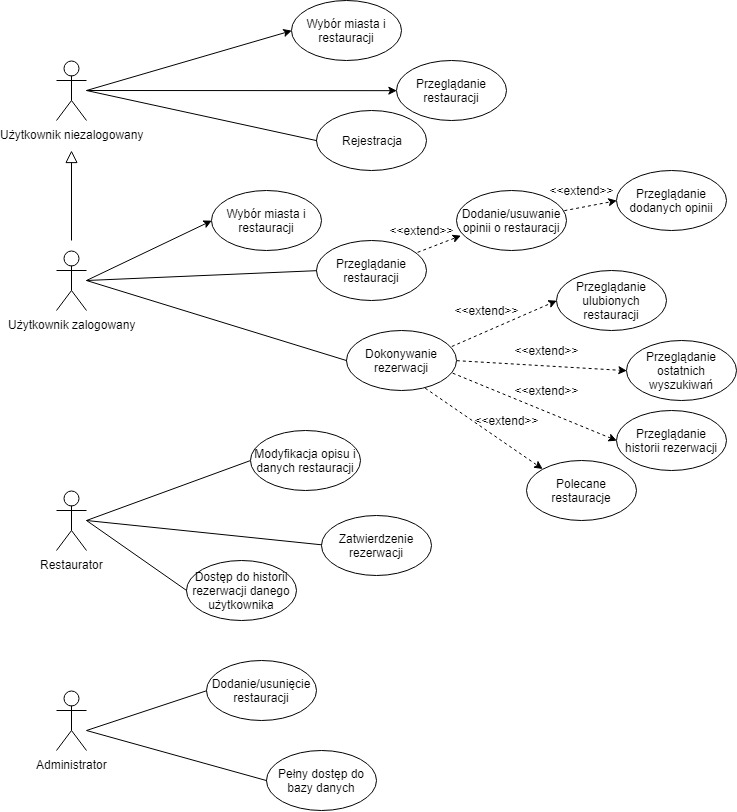
\includegraphics[width=0.90\textwidth]{use_case.jpg}
	\caption{Schemat przypadków użycia systemu.}
\end{figure}

\subsubsection{Podstawowe przypadki użycia}



\subsection{Wymagania niefunkcjonalne}

\subsubsection{Wykorzystane technologie i narzędzia}

Projekt został zrealizowany z wykorzystaniem języka C\# oraz frameworka ASP.NET MVC. Do realizacji frontendu zostały wykorzystane HTML5, CSS 3.0 oraz JavaScript. Jako system zarządzania bazą danych wykorzystano Microsoft SQL Server.

\begin{figure}
\centering
		\begin{minipage}{2cm}
			
\includegraphics[width=2cm]{c_hasztag.png}
		\end{minipage}
		\begin{minipage}{2cm}
			
\includegraphics[width=2cm]{asp_net-MVC.png}
		\end{minipage}
		\begin{minipage}{2cm}
			
\includegraphics[width=2cm]{html.png}
		\end{minipage}
		\begin{minipage}{2cm}
			
\includegraphics[width=2cm]{sql.png}
		\end{minipage}
	\caption{Wykorzystane technologie.}
	\label{fig:technologie}
\end{figure}

\begin{figure}
\centering
	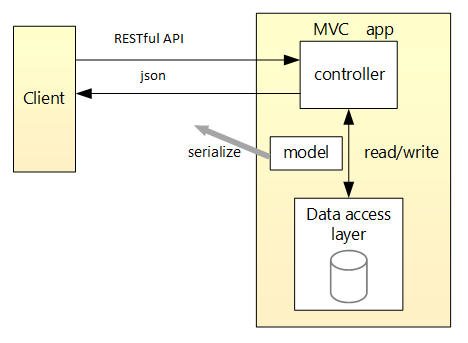
\includegraphics{mvc.png}
	\caption{Podstawowy schemat działania aplikacji korzystającej z .NET MVC.}
\end{figure}

\section{Projekt systemu}

\subsection{Architektura systemu}



\section{Podsumowanie i wnioski}


\end{document}